\documentclass[12pt]{article}
\usepackage{graphicx} 
\usepackage{amsmath}
\usepackage{amsthm}
\usepackage{graphicx}
\usepackage{enumerate}
\usepackage{natbib}
\usepackage{booktabs}
\usepackage{hyperref}
\hypersetup{colorlinks = true, linkcolor = blue, citecolor=blue, urlcolor = blue}
\usepackage{enumitem}
\newcommand{\blind}{0}
\addtolength{\oddsidemargin}{-.5in}%
\addtolength{\evensidemargin}{-.5in}%
\addtolength{\textwidth}{1in}%
\addtolength{\textheight}{1.3in}%
\addtolength{\topmargin}{-.8in}%
\usepackage{float}
\usepackage{array} 



\begin{document}



\def\spacingset#1{\renewcommand{\baselinestretch}%
{#1}\small\normalsize} \spacingset{1}


%%%%%%%%%%%%%%%%%%%%%%%%%%%%%%%%%%%%%%%%%%%%%%%%%%%%%%%%%%%%%%%%%%%%%%%%%%%%%%

\if0\blind
{
  \title{\bf The usage of bootstrap method in shape-restricted regression}
  \author{Guanghong Yi\\
  Jun Yan\\[1ex]
  Department of Statistics, University of Connecticut\\
}
  \maketitle
} \fi

\if1\blind
{
  \bigskip
  \bigskip
  \bigskip
  \begin{center}
    {\LARGE\bf The usage of bootstrap method in shape-restricted regression}
\end{center}
  \medskip
} \fi

\bigskip
\begin{abstract}
The bootstrap method is an important resampling technique used to estimate 
statistics on a population by repeatedly sampling the data. It is also an 
effective approach for estimating the measure of dispersion in a dataset, 
especially in regression analysis. Meanwhile, the bootstrap method is also
a valid method for constructing pointwise confidence intervals for time 
points in regressions. However, in some special cases, regression models 
need to be constrained with known characteristics such as monotonicity or
curvature, for example, in growth curves, where the coefficients are 
forced to be non-negative. In such situations, spline regression is used
for modeling. It is not always certain whether the bootstrap method can 
be directly applied to estimate the dispersion under these shape-restricted
scenarios, especially for pointwise confidence intervals. In this article,
we will demonstrate the usage of the bootstrap method in shape-restricted 
regression and proof the effectiveness of bootstrap for constructing 
pointwise confidence intervals in shape-restricted regression empirically.
\end{abstract}

\noindent%
{\it Keywords:}  bootstrap; shape-restricted regression; 
pointwise confidence interval; growth curve; splines regression
\vfill

\newpage
\spacingset{1.45} 
\section{Introduction}
\label{sec:intro}

Bootstrap is a powerful and important resampling method for estimating population
parameters or assessing the accuracy of a statistical procedure by repeatedly 
sampling the data with replacement. Its effectiveness have been widely recognized
in linear regression analysis \cite{efron1979bootstrap}, and non-linear regression
analysis \cite{davidson1999bootstrap}. By bootstrap method, we can estimate the 
standard errors of the regression coefficients. Even for unknown underlying 
population distributions, bootstrap method can resample the data with replacement 
and computes the regression coefficients for each resampled dataset. 
\cite{hall2013simple}By repeating this process many times, it provides a valid 
empirical estimate of the standard errors in both linear cases 
\cite{efron1985bootstrap} and nonlinear cases\cite{wong2019bootstrap}, thus it is
valuable when the assumptions of traditional standard error estimation techniques 
are violated. It is also a valid method used to construct confidence intervals for
regression coefficients. \cite{efron1985bootstrap}By resampling the dataset, 
bootstrap can determining the percentile intervals of these coefficients, and also
can obtain approximate confidence intervals for the regression parameters. 
\cite{cui2012evaluating} Bootstrap can also construct the approximate confidence 
interval for certain time points f(t)s in the function by simulating f'(t) certain
times in certain time points. \cite{horowitz2018bootstrap} However, when dealing 
with shape-restricted regressions, where the coefficients are forced to adhere to 
specific constraints such as monotonicity or curvature, the effectiveness of 
bootstrap is not proved to be guaranteed. In this paper, we will demonstrate the
usage of the bootstrap method in shape-restricted regression and proof the 
effectiveness of bootstrap for constructing pointwise confidence intervals in 
shape-restricted regression empirically.


The rest of the paper is organized as the follows. 
Section~\ref{Bootstrap Method for Constructing Confidence Intervals}
gives a review of bootstrap method for constructing confidence intervals. 
Section~\ref{Shape Restricted Example} gives out a shape-restricted regression
example and the usage of bootstrap to build the pointwise confidence intervals 
for certain time points. Section~\ref{Simulation Study} shows a simulation study
to assess the performance of the methods.
explores the case where a combination of the first two scenarios occurs. An  
adjusted bootstrap procedure is proposed as a working solution in this case.  
Section~\ref{Conclusion} concludes with a discussion.




\section{Bootstrap Method for Constructing Confidence Intervals}
\label{Bootstrap Method for Constructing Confidence Intervals}

The bootstrap method is a powerful resampling technique used to construct 
confidence intervals for population parameters or estimates when the underlying 
distribution is unknown or difficult to determine. \cite{hall2013simple}It is 
useful in regression analysis to estimate the uncertainty associated with the 
regression coefficients or for certain time points inside the regression 
function. Specifically, the bootstrap method basically contains three steps:

\begin{enumerate}[label=\arabic*.]
    \item Let \(v\) represent a population parameter of interest (e.g., mean,
    median, standard deviation, etc.), which is drawn from an unknown population
    distribution \(F\).
    \item Generate a bootstrap sample \(x_1, x_2, \ldots, x_n\) from the 
    population, and they are referred to as the original sample dataset.
    \item Let \(u\) represent a statistic calculated from the bootstrap original
    sample dataset.
    \item Using the data in the original sample dataset as the "population," 
    perform nonparametric resampling with replacement to obtain a resampled sample
    (also known as the Bootstrap sample), denoted as \(x_1^*, x_2^*, \ldots, x_n^*\)
    (the number of data points in the Bootstrap sample must be the same as the 
    number of data points in the original sample).
    \item Let \(u^*\) represent the statistic computed by the Bootstrap 
    sample datasets, and this will be the bootstrap estimated statistic 
    for the population statistic.

\end{enumerate}

Bootstrap method has been proved that it is an excellent method to estimate 
statistic \cite{efron1979bootstrap}, the \(u^*\) we obtained from the resampling
dataset is a good estimator for the \(v\) as a population parameter. According 
to the bootstrap method, we can also calculate the confidence interval for the 
parameters, or the coefficients of a certain regression, or for certain time points
in the regression. In this article, we will focus on the method of construct a 
pointwise confidence interval by bootstrap. To construct a pointwise confidence 
interval using the bootstrap method, the procedure involves the following steps:

\begin{enumerate}[label=\arabic*.]
    \item First we observed a specific time point \(t\) that we are interested 
    and its corresponding true value \(f(t)\), and build them as a pair \(t, f(t)\).
    \item According to the dataset, fit \(\hat{f}\) as the estimated regression for
    the dataset.
    \item Generate a bootstrap sample \(x_1, x_2, \ldots, x_n\) from the population
    by sampling with replacement, and they are referred to as the original sample
    dataset. 
    \item Then  
    \( [\hat{f}_n(t) - \hat{q}_{1-\alpha/2,n-1/3}, \hat{f}_n(t) - \hat{q}_{\alpha/2,n-1/3} ]\)
    would be the bootstrap estimated pointwise confidence interval 
    where \(\hat{q}_\alpha\) denoted the \(\alpha\)th quantile of the time point \(t\).

\end{enumerate}





It has been proved that the bootstrap method can be used as a good estimator for
the pointwise confidence interval in linear regressions and non-linear regressions
\cite{efron1979bootstrap}\cite{davidson1999bootstrap}, and some examples in certain
configurations are given.\cite{ruhe2019bootstrap}\cite{ma2019inference}
\cite{dugas2010pointwise} But in certain special cases(i.e. shape-restricted splines 
regressions) there is no certain resource have not prove that it is a good method to
build pointwise confidence interval via bootstrap.

Shape-restricted splines regressions are piecewise polynominal, differentiable to a
certain degree and have certain restrictions like monotonicity or convexity.
\cite{meyer2008inference} Given these conditions, the application of the bootstrap
method to estimate pointwise confidence intervals for specific time points within 
the regression cannot be guaranteed to be suitable. And in the rest of the article
we gives out an example of shape-restricted regression and the method to fit confidence
interval for certain time points in the function.









\section{Shape Restricted Example}
\label{Shape Restricted Example}

In some situations the regression is forced to be shape-restricted to improve
the predictive performance and reduce overfitting if the underlying regression 
function takes the specific form. Some regressions are naturally constrained to
convexity or concativity in a lot of disciplines like economics, biology, and 
psychological studies, and other ares.\cite{jieying2022heteroscedastic} 
\cite{guntuboyina2018nonparametric} Some popular examples like cost function and 
profit function in economics\cite{gallant1984imposing}, precipitation data analysis
\cite{molitor2002bayesian}. In this article we gives out an example of the 
relationship between income and the age of Canadian workers. The data is given from
R package SemiPar. For those situations, Regression splines are smooth, flexible, 
and parsimonious nonparametric function estimators, and it offers an effective approach
to enhance the inference of shape-restricted regression. \cite{meyer2008inference} 
In this dataset, a nondecreasing relationship between the age of workers and the 
expected logarithm of the income was considered. \cite{wang2021shape}  Splines2 provides
implementation of those spline basis functions via R language, and we use that to build 
a non-decreasing curve by i-spline that force the coefficients to be non-negative with
degree of freedom = 6. Then, we selected 10 time points, denoted as $t$, with equal 
intervals from the dataset, corresponding to one of them is the regression time points
\(f'(t)\) that fitted by iSpline. We also performed bootstrap resampling 1000 times to
obtain the 95\% quantile pointwise confidence interval for each points. In the figure
below, the red line represents the fitted i-spline regression, the yellow line is the
smooth regression, and we build ten pointwise confidence intervals for 10 certain time
points. The result is shown in Figure ~\ref{fig:semipar}.


\begin{figure}[H]
  \centering
  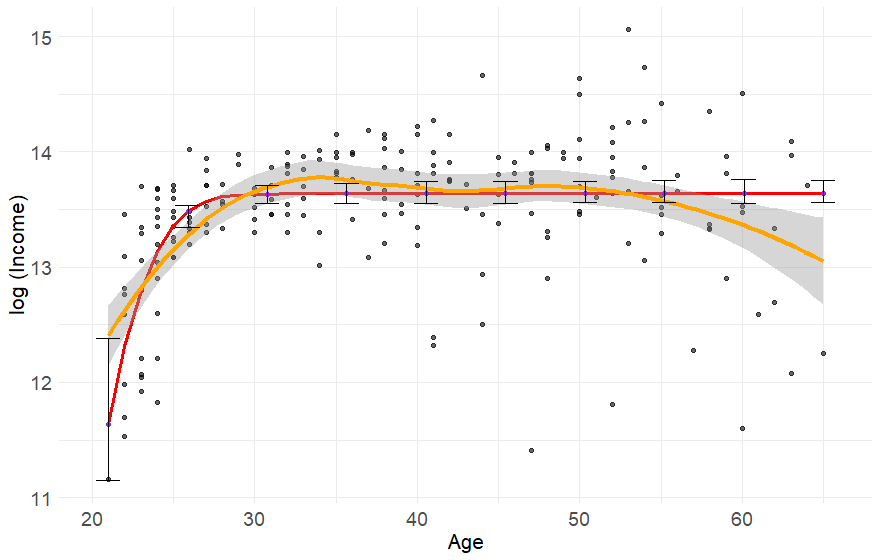
\includegraphics[width=0.8\textwidth]{SemiparCI.png}
  \caption{CI build for the shape-restricted regression: The red line is the 
  fitted i-splines regression, the yellow line is the smoothing splines, the
  grey area represents the \(95\%\) confidence interval for the smoothing splines, 
  and the black solid intervals are the bootstrap pointwise confidence intervals for
  certain time points. }
  \label{fig:semipar}
\end{figure}

We can see that, for this one-time example all the pointwise confidence intervals 
constructed by the bootstrap method include the fitted regression. But it is not a
valid proof that bootstrap is a good method for constructing pointwise confidence 
intervals since the regression is fitted by the dataset, and the criteria is given
by \(f'(t)\) which is given by the regression but not the the true value \(f(t)\).
In this case, a simulation study is required to further prove the effectiveness of 
bootstrap pointwise confidence intervals.









\section{Simulation Study}
\label{Simulation Study}


Since the underlying distribution is unknown, we need to perform a simulation
study to test whether the fitted pointwise confidence interval is accurate 
for the regression.


We define three functions: \(y = 0.25(x - 0.9)\) , \(y = 0.02(x^3+1.2)\) , and
\( y = 0.1 (5\Phi((x - 2) / 0.3) + 1)\) , where \(\Phi\) is the cumulative 
distribution function of the standard normal distribution. For those functions,
the validity of the bootstrap method to build the confidence intervals for the
coefficients and standard error has already been proved. 
\cite{jieying2022heteroscedastic} And in this article we want to further prove
the validity of the bootstrap method to build the pointwise confidence intervals
for certain time points in the domain of the function. First of all, we randomly
generate 1000 points \(x\) in the domain of \([0,30]\), and we calculate its 
corresponding values \(y(x)\), and make simulation data points \(f'(x)\) by add 
noise to the true value \(f(x)\). The noise is added from a standard normal 
distribution with \(\mu = 0\) and \(\sigma = \) \(1\). And then we make the 
paired values \((x, y\text{ with noise})\) be the dataset, while we know the 
true values of \(f(x)\) as well. 


\begin{figure}[H]
  \centering
  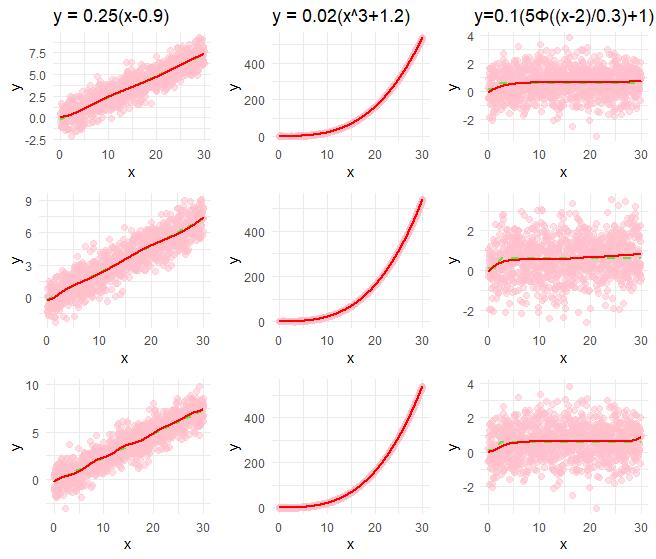
\includegraphics[width=0.8\textwidth]{DataAndRegressions.png}
  \caption{The generated dataset, true functions and fitted i-splines regressions
  : the shaded green curve represents the true functions, the pink points are the
  data pair \((x, f'(x))\) where \(f'(x)\) is generated by \(f(x)\) add noise,
  and the red curves are the fitted i-splines regression curve with degrees of 
  freedom\(= 6,10,15\), from top to bottom}
  \label{fig:DataAndRegressions}
\end{figure}

We use quadratic i-splines function to enforce the monotonicity of the function
and we picked degrees of freedom 6,10,15 to build the regression for the dataset.
The generated dataset and regressions is shown in Figure 
~\ref{fig:DataAndRegressions}. In each configuration, we select 1, 5, 10, 15, 20,
25, 30 as the time points from the dataset and perform bootstrap resampling 1000 
times to estimate the \(95\%\) quantile pointwise confidence intervals for each 
of the selected time points. We repeat this process 1000 times to see how many 
times these confidence intervals can contain the true result. The results are 
shown in Table ~\ref{Table}. 



\begin{table}[ht]
  \centering
  \label{Table}
  \caption{Results of functions for different degrees of freedom}
  \begin{tabular}{|c|c|c|c|c|}
    \hline
    \textbf{x} & \textbf{f(x)} & \textbf{CP of df\_6} & \textbf{CP of df\_10} & \textbf{CP of df\_15} \\
    \hline
    \multicolumn{5}{|c|}{\(y = 0.25(x - 0.9)\)} \\
    \hline
    1 & 0.025 & 0.936 & 0.944 & 0.939 \\
    \hline
    5 & 1.025 & 0.960 & 0.958 & 0.948 \\
    \hline
    10 & 2.275 & 0.956 & 0.950 & 0.951 \\
    \hline
    15 & 3.525 & 0.959 & 0.954 & 0.954 \\
    \hline
    20 & 4.775 & 0.941 & 0.949 & 0.961 \\
    \hline
    25 & 6.025 & 0.953 & 0.946 & 0.942 \\
    \hline
    30 & 7.275 & 0.919 & 0.955 & 0.947 \\
    \hline
    \multicolumn{5}{|c|}{\(y = 0.02(x^3+1.2)\)} \\
    \hline
    1 & 0.025 & 0.893 & 0.940 & 0.959 \\
    \hline
    5 & 1.025 & 0.932 & 0.948 & 0.958 \\
    \hline
    10 & 2.275 & 0.937 & 0.948 & 0.941 \\
    \hline
    15 & 3.525 & 0.942 & 0.951 & 0.953 \\
    \hline
    20 & 4.775 & 0.939 & 0.951 & 0.957 \\
    \hline
    25 & 6.025 & 0.952 & 0.959 & 0.963 \\
    \hline
    30 & 7.275 & 0.947 & 0.943 & 0.943 \\
    \hline
    \multicolumn{5}{|c|}{\(y = 0.1 (5\Phi((x - 2) / 0.3) + 1)\)} \\
    \hline
    1 & 0.025 & 0.686 & 0.847 & 0.901 \\
    \hline
    5 & 1.025 & 0.279 & 0.800 & 0.852 \\
    \hline
    10 & 2.275 & 0.947 & 0.937 & 0.942 \\
    \hline
    15 & 3.525 & 0.937 & 0.953 & 0.961 \\
    \hline
    20 & 4.775 & 0.929 & 0.950 & 0.957 \\
    \hline
    25 & 6.025 & 0.953 & 0.924 & 0.922 \\
    \hline
    30 & 7.275 & 0.919 & 0.858 & 0.832 \\
    \hline
  \end{tabular}
\end{table}

In table ~\ref{Table}, \(x\) represents the certain time point we 
selected in the domain of the function, and \(f(x)\) is its true value
calculated by the certain known function. CP represents coverage
percentage of pointwise confidence interval we built by the bootstrap 
methods under certain degrees of freedom. We can see that in all those 
functions and degrees of freedom we have given, the bootstrap method 
gives pointwise confidence intervals coverage that are closed to the 
nominal level \(95\%\).


\section{Conclusion}
\label{Conclusion}
In this study, we explored the application of the bootstrap method of 
building pointwise confidence intervals in shape-restricted cases. 
We demonstrated its effectiveness in constructing pointwise confidence
intervals for certain time points within the regression function. 

We gives out a simulation study to prove that the pointwise confidence
intervals constructed using the bootstrap method provide good 
empirical coverage for the true values of the regression function. 
This suggests that the bootstrap method is a valid approach for 
enhancing the inference of shape-restricted regressions, even for 
pointwise confidence intervals.

Our findings support the utility of the bootstrap method to build
the pointwise confidence intervals in cases where regression models
have specific constraints such as monotonicity or curvature. However
, it's important to consider the assumptions and limitations of the
bootstrap method and validate its performance for specific datasets and applications.

\bibliographystyle{plain}
\bibliography{citations}


\end{document}
